\documentclass[12pt]{article}

\usepackage[a4paper, margin=1in]{geometry}
\usepackage{graphicx}
\usepackage[absolute, overlay]{textpos}
\usepackage{fancyhdr}
\usepackage{siunitx}
\usepackage{tikz}
\usepackage{pgfplots}
\usetikzlibrary{decorations.pathmorphing}
\usetikzlibrary{math}
\usetikzlibrary{calc}

\pgfplotsset{compat=1.18}

\pagestyle{fancy} %for footers

\newcommand{\customsubject}{}   
\newcommand{\customtitle}{}

\newcounter{questionpartcounter}                  %Setup for question part counter for a,b,c listing
\renewcommand{\thequestionpartcounter}
{\alph{questionpartcounter}}

\newcounter{questionpartpartcounter}                  %Setup for question part  partcounter for a,b,c listing
\renewcommand{\thequestionpartpartcounter}
{\roman{questionpartcounter}}

\pagestyle{fancy} %for footers
\renewcommand{\headrulewidth}{0pt}
\fancyhf{}
\fancyfoot[R]{\thepage}

\newenvironment{worksheet}[2]
{
    
    \global\renewcommand{\customtitle}{#1}
    \global\renewcommand{\customsubject}{#2}


    \begin{textblock*}{5cm}(0.4cm,0.4cm)
   
\includegraphics[width=4cm]{include/figures/bmdwlogo}
\end{textblock*}

    \vspace*{-1cm}
    
    {\large\textbf{\begin{center}\customtitle\end{center}}}

    \begin{center}\customsubject\end{center}
    
    \vspace{0.3cm}
    
    \hspace*{-1.5cm}\textbf{Name:\ \rule{4cm}{0.4pt}}\; 
    \textbf{Student \#: \ \rule{3cm}{0.4pt}}\;
    \textbf{Student Email \#: \ \rule{1.53cm}{0.4pt}}

    \vspace{0.5cm}

    
    \begin{enumerate}
}
{
    \end{enumerate}
   % \begin{textblock*}{10cm}(1cm, 28cm) {\footnotesize \scriptsize \customsubject}
    
%\end{textblock*}
}



\newcommand{\question}[2][1cm]{%
    \item
    \setcounter{questionpartcounter}{0}
    \setcounter{questionpartpartcounter}{0}
    {#2}
    \vspace{#1}
}

\newcommand{\questionpart}[2][1cm]{%
    \setcounter{questionpartpartcounter}{0}
    \stepcounter{questionpartcounter}
    (\thequestionpartcounter)~#2
    \vspace{#1}
}

\newcommand{\questionpartpart}[2][1cm]{%
      \stepcounter{questionpartpartcounter}
      \thequestionpartpartcounter.~#2
      \vspace{#1}
}

\newcommand{\operation}[1]{%
{\large $
#1
$}
}



\begin{document}

\begin{worksheet}{Physics Worksheet}{Integral Practice}


%Basic question
\question[4.5cm]{Compute:  \vspace{-1cm}\begin{eqnarray*}\displaystyle \int 3x^2 + \frac{1}{x} + e^x \; dx \end{eqnarray*}}




%infinite sum
\question[0.5cm]{Ari is running with an inital velocity of \SI{1}{\metre\per\second} and an acceleration of $\frac{1}{5}x^4$ \SI{}{\metre\per\second\squared}}

\questionpart[5cm]{How fast will ari be going after 5 seconds of running? Answer in the form of an infinite sum}

\questionpart[0cm]{Construct and compute an integral to find the exact value}


\newpage

%Conceptual question
\question[0.25cm]{Below is the function $f(x) = -x^2 +9$}
\\
\questionpart[0.5cm]{Using the grid, approximate the area under the curve with increasing accuracy}

\hspace{-3.5cm}
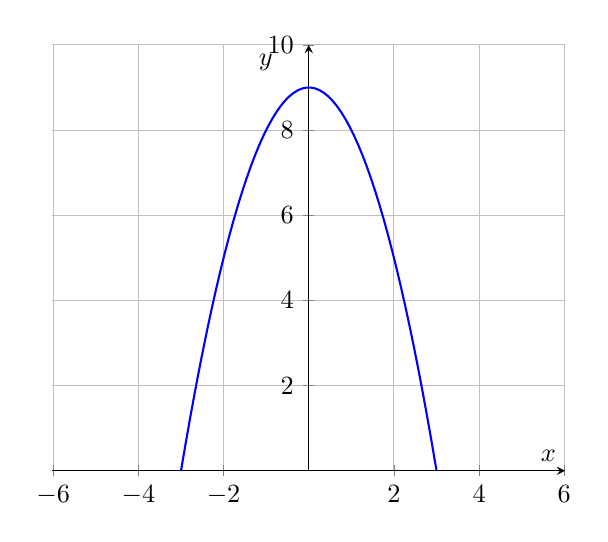
\begin{tikzpicture}[scale=0.95]
  \begin{axis}[
    axis lines = middle,
    xlabel = $x$,
    ylabel = {\hspace{-1.2cm}$y$},
    xmin=-3, xmax=3,
    ymin=0, ymax=10,
    samples=100,
axis equal,
    grid=both,
  ]
    \addplot[blue, thick] {-x^2 + 9};
  \end{axis}
\end{tikzpicture}
\hspace{0cm}
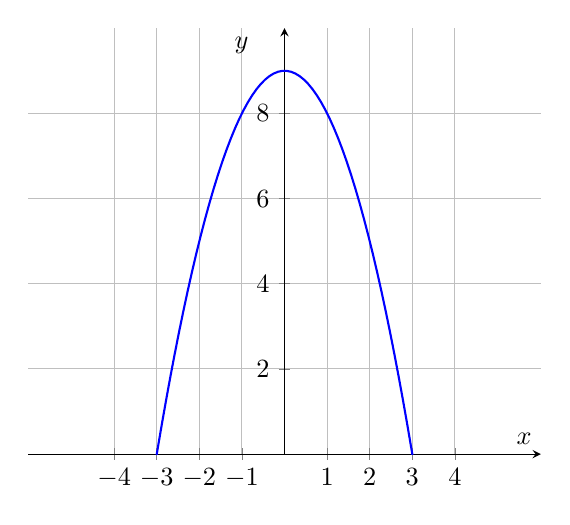
\begin{tikzpicture}[scale=0.95]
  \begin{axis}[
    axis lines = middle,
    xlabel = $x$,
    ylabel = {\hspace{-1.2cm}$y$},
    xmin=-3, xmax=3,
    ymin=0, ymax=10,
    xtick={-4,-3,-2,-1,0,1,2,3,4},
    ytick={0,2,4,6,8},
    samples=100,
axis equal,
    grid=both,
  ]
    \addplot[blue, thick] {-x^2 + 9};
  \end{axis}
\end{tikzpicture}
\hspace{0cm}
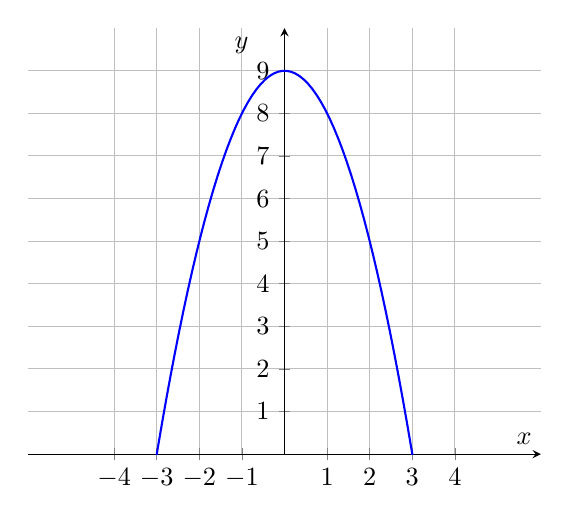
\begin{tikzpicture}[scale=0.95]
  \begin{axis}[
    axis lines = middle,
    xlabel = $x$,
    ylabel = {\hspace{-1.2cm}$y$},
    xmin=-3, xmax=3,
    ymin=0, ymax=10,
    xtick={-4,-3,-2,-1,0,1,2,3,4},
    ytick={0,1,2,3,4,5,6,7,8,9},
    samples=100,
axis equal,
    grid=both,
  ]
    \addplot[blue, thick] {-x^2 + 9};
  \end{axis}
\end{tikzpicture}
\vspace{2.5cm}

\questionpart[4.5cm]{Find the true value of the area under the curve by computing $\displaystyle \int_{-3}^{3} (-x^2 + 9) \; dx$}



%Derivation question
\question[0cm]{Derive: $\displaystyle x = x_0 +v_i t + \frac{1}{2}at^2$}















\end{worksheet}

\end{document}